\chapter{Radar}
A radar, well what does it do and why we use it? 

The challenge of seeing objects and estimating a distance to these objects, has been vastly minimized by the invention of the radar. Not only does the radar tell you that there is an object, but it also tells you in which direction and at what distance the object is. This has shown to be very use full onboard ships and aeroplanes, but also on land, at stations monitoring ship and air traffic, airports etc. While placed on land, the main purpose of the radar is to detect ship traffic and air traffic. But when a radar is placed on for example a ship, its main purpose is to detect other ships and/or objects within the sailing path, so that the ship doesn't collide, it prevents accidents. 

The radar is the eyes and ears of the navigator. It has a 360-degree view and can detect moving objects as well as still standing objects. It gives you the direction, distance and speed of the object, no matter how big or small the object is, but of course depending on the type of radar and the use.  

A radar is based on a radio transmitter and a receiver, therefore the name radar (Radio Detection And Ranging). It uses a very high frequency, much higher than any television or radio signal, this to prevent distortion from other radio signals. When in function it sends out small electromagnetic pulses, through an antenna, and if this pulse hits anything, the echo gets sent back for the receiver to pick up, very much like how a bat finds its way in the dark. There do exist many types of radar, one for each specific use. The angle of which the transmitter sends out the pulse, decides the use of the radar, for example does an airport radar point upwards, since it detects air traffic and a ship radar is used to detect objects at the same level as the ship.

\section{Hardware components}
\begin{itemize}
  \item LED
  \item RGB LED
  \item Push button
  \item LCD Display
  \item Temperature sensor 
  \item Servo Motor 
  \item Ultrasonic sensor
  \item Resistors
\end{itemize}

\section{ Hardware components purpose and what are they being used for}

\subsection{LED}

\begin{figure} [h!]
\centering
  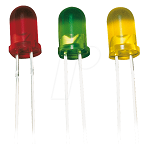
\includegraphics{fig/LEDperur}
  \caption{LEDS}
  \label{fig:LEDS}
\end{figure}

A LED (light-emitting diode) is used like a small light bulb, but is in fact a semiconductor, since it only lets current flow in one direction, from the anode to the cathode. It is used for many purposes in today's society, especially for lighting, regular light bulbs and Christmas lights, but also for back light in televisions. When working with Arduino you can make this small LED to light up constantly or to flash, depending on what purpose it serves. 

In this project the LED, well in fact there are three LED's (green, yellow and red), their purpose is to indicate whether the radar is on, off or loading, depending on the state of the push button. 

\subsection{RGB LED}

\begin{figure} [h!]
\centering
  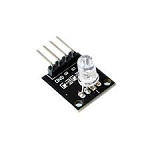
\includegraphics{fig/RGBLED}
  \caption{RGB LED}
  \label{fig:RGBLED}
\end{figure}

A RGB LED is much like a regular LED, but the main difference being that the RGB LED can change colour, meaning that it consists of three LED's with the standard colours red, green and blue. The brightness of each LED decides the colour of the LED, much like mixing paint, but using light instead of paint. 

The RGB LED used indicates at what distance the object detected by the Ultra Sonic is, so if the light of the RGB LED turns red the object is closer than 10 cm, if it turns green the object is between 10 cm to 100 cm and when it's blue the object is at a distance of a 100 cm or more.  

\subsection{Push button}

\begin{figure} [h!]
\centering
  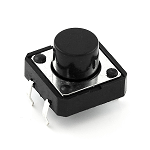
\includegraphics{fig/Pushbutton}
  \caption{Push button}
  \label{fig:Pushbutton}
\end{figure}

A push button reassembles a light switch in our home. When the button is not pressed it does not let any current through it, known as state HIGH in the programming. When the button gets pressed, it lets current flow through it, much like when a light switch is on, the state is known as LOW. 

The purpose of the button used is to turn the radar on and off, that means when the radar is off the red LED is lit and nothing moves. And when the button is pressed, the green LED is lit and the Radar is moving.

\subsection{LCD display}

\begin{figure} [h!]
\centering
  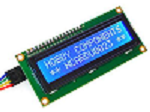
\includegraphics{fig/LCDdisplay}
  \caption{LCD Display}
  \label{fig:LCDdisplay}
\end{figure}  

The LCD display (liquid crystal display) is a very common thing, displays are used in everything from televisions to cell phones. The one for the Arduino is a very simple one, it doesn't come with colour, meaning the writing is white, and it is only capable of writing two lines, containing 16 signs in each line, it mostly resembles the old cell phones.   

Regarding the project, when the radar is turned off the display reads ``Radar project version $2.0$''. When turning the radar on the display clears and starts displaying the direction of the Servo Motor and Ultra Sonic. When the Ultra Sonic detects an object, the display shows at what distance the object is and at what angle from the radar. It also displays the temperature measured, by the temperature measurer, since the temperature has an effect on the speed of sound. 

\subsection{Temperature sensor}

\begin{figure} [h!]
\centering
  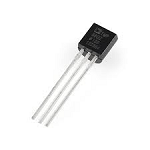
\includegraphics{fig/Temperaturesensor}
  \caption{Temperature sensor}
  \label{fig:temperaturesensor}
\end{figure} 

The temperature sensors job is to measure the temperature of the surroundings, since the speed of sound and temperature go hand in hand. 

\subsection{Servo motor}

\begin{figure} [h!]
\centering
  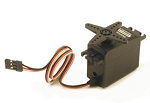
\includegraphics{fig/Servomotor}
  \caption{Servo motor}
  \label{fig:servo}
\end{figure} 

A servo motor is based on an Arduino library, which is included in the Arduino, the library is the used in the programming. On the hardware part, the servo motor has integrated gears and shaft, which allows it to be controlled precisely. The standard servo motor can be positioned at various angles between $0$ to $180$ degrees. 

The purpose of the Servo Motor is to turn the Ultrasonic sensor in an arc of $180$ degrees, from left to right and back. Its job is also to let the user and Arduino know at all times at what angle it's located. This information is used to tell at what angel an object is located. 


\subsection{Ultrasonic sensor}

\begin{figure} [h!]
\centering
  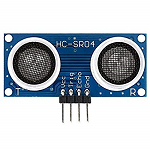
\includegraphics{fig/Ultrasonicsensor}
  \caption{Ultrasonic sensor}
  \label{fig:ultrasonic}
\end{figure}

The Ultrasonic sensor is based on sonar technology and can determine the distance of an object, with a range of $2 cm$ to $400 cm$. It doesn't get affected by sunlight and comes as a complete module, including the transmitter and receiver.  

In this case the ultrasonic sensor is placed on the moving servo motor, so it can detect objects in a 180-degree radius, thereby being able to see what is in front, it is the key component of the radar. By detecting an object and at what distance, it gives us an idea of where and how close in front of us an object is located.   

\subsection{Resistors}

\begin{figure} [h!]
\centering
  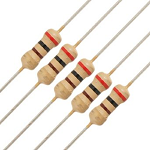
\includegraphics{fig/Resistor}
  \caption{Resistors}
  \label{fig:Resistors}
\end{figure}

The resistors help control the current flowing to different components, meaning the limit the amount of current flowing to the components. This becomes much needed when working with highly current sensitive components, like the LED's, which can only withstand $2 V$. However, it is also used in front of the push button to direct the current, to detect if the button is pressed down or not.

\section{Complete circuit}

\begin{figure} [h!]
\centering
  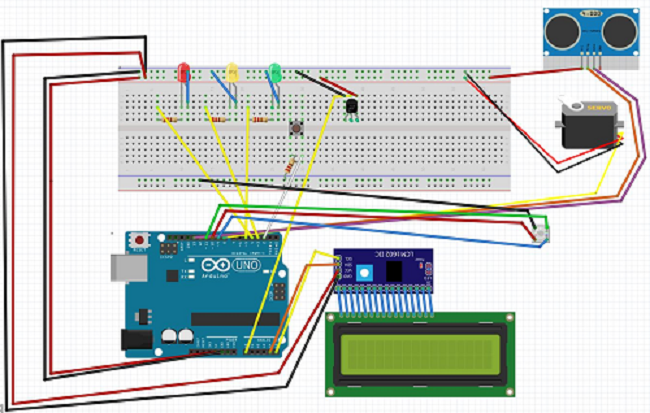
\includegraphics [width=\linewidth]{fig/Arduinoboard}
  \caption{Arduino drawing}
  \label{fig:Arduinoboard}
\end{figure}

On the picture it looks like everything is connected to each other and in a way it is, since the board itself is what brings everything together. But we can simplify it into this electrical drawing: 

\newpage

\begin{figure} [h!]
\centering
  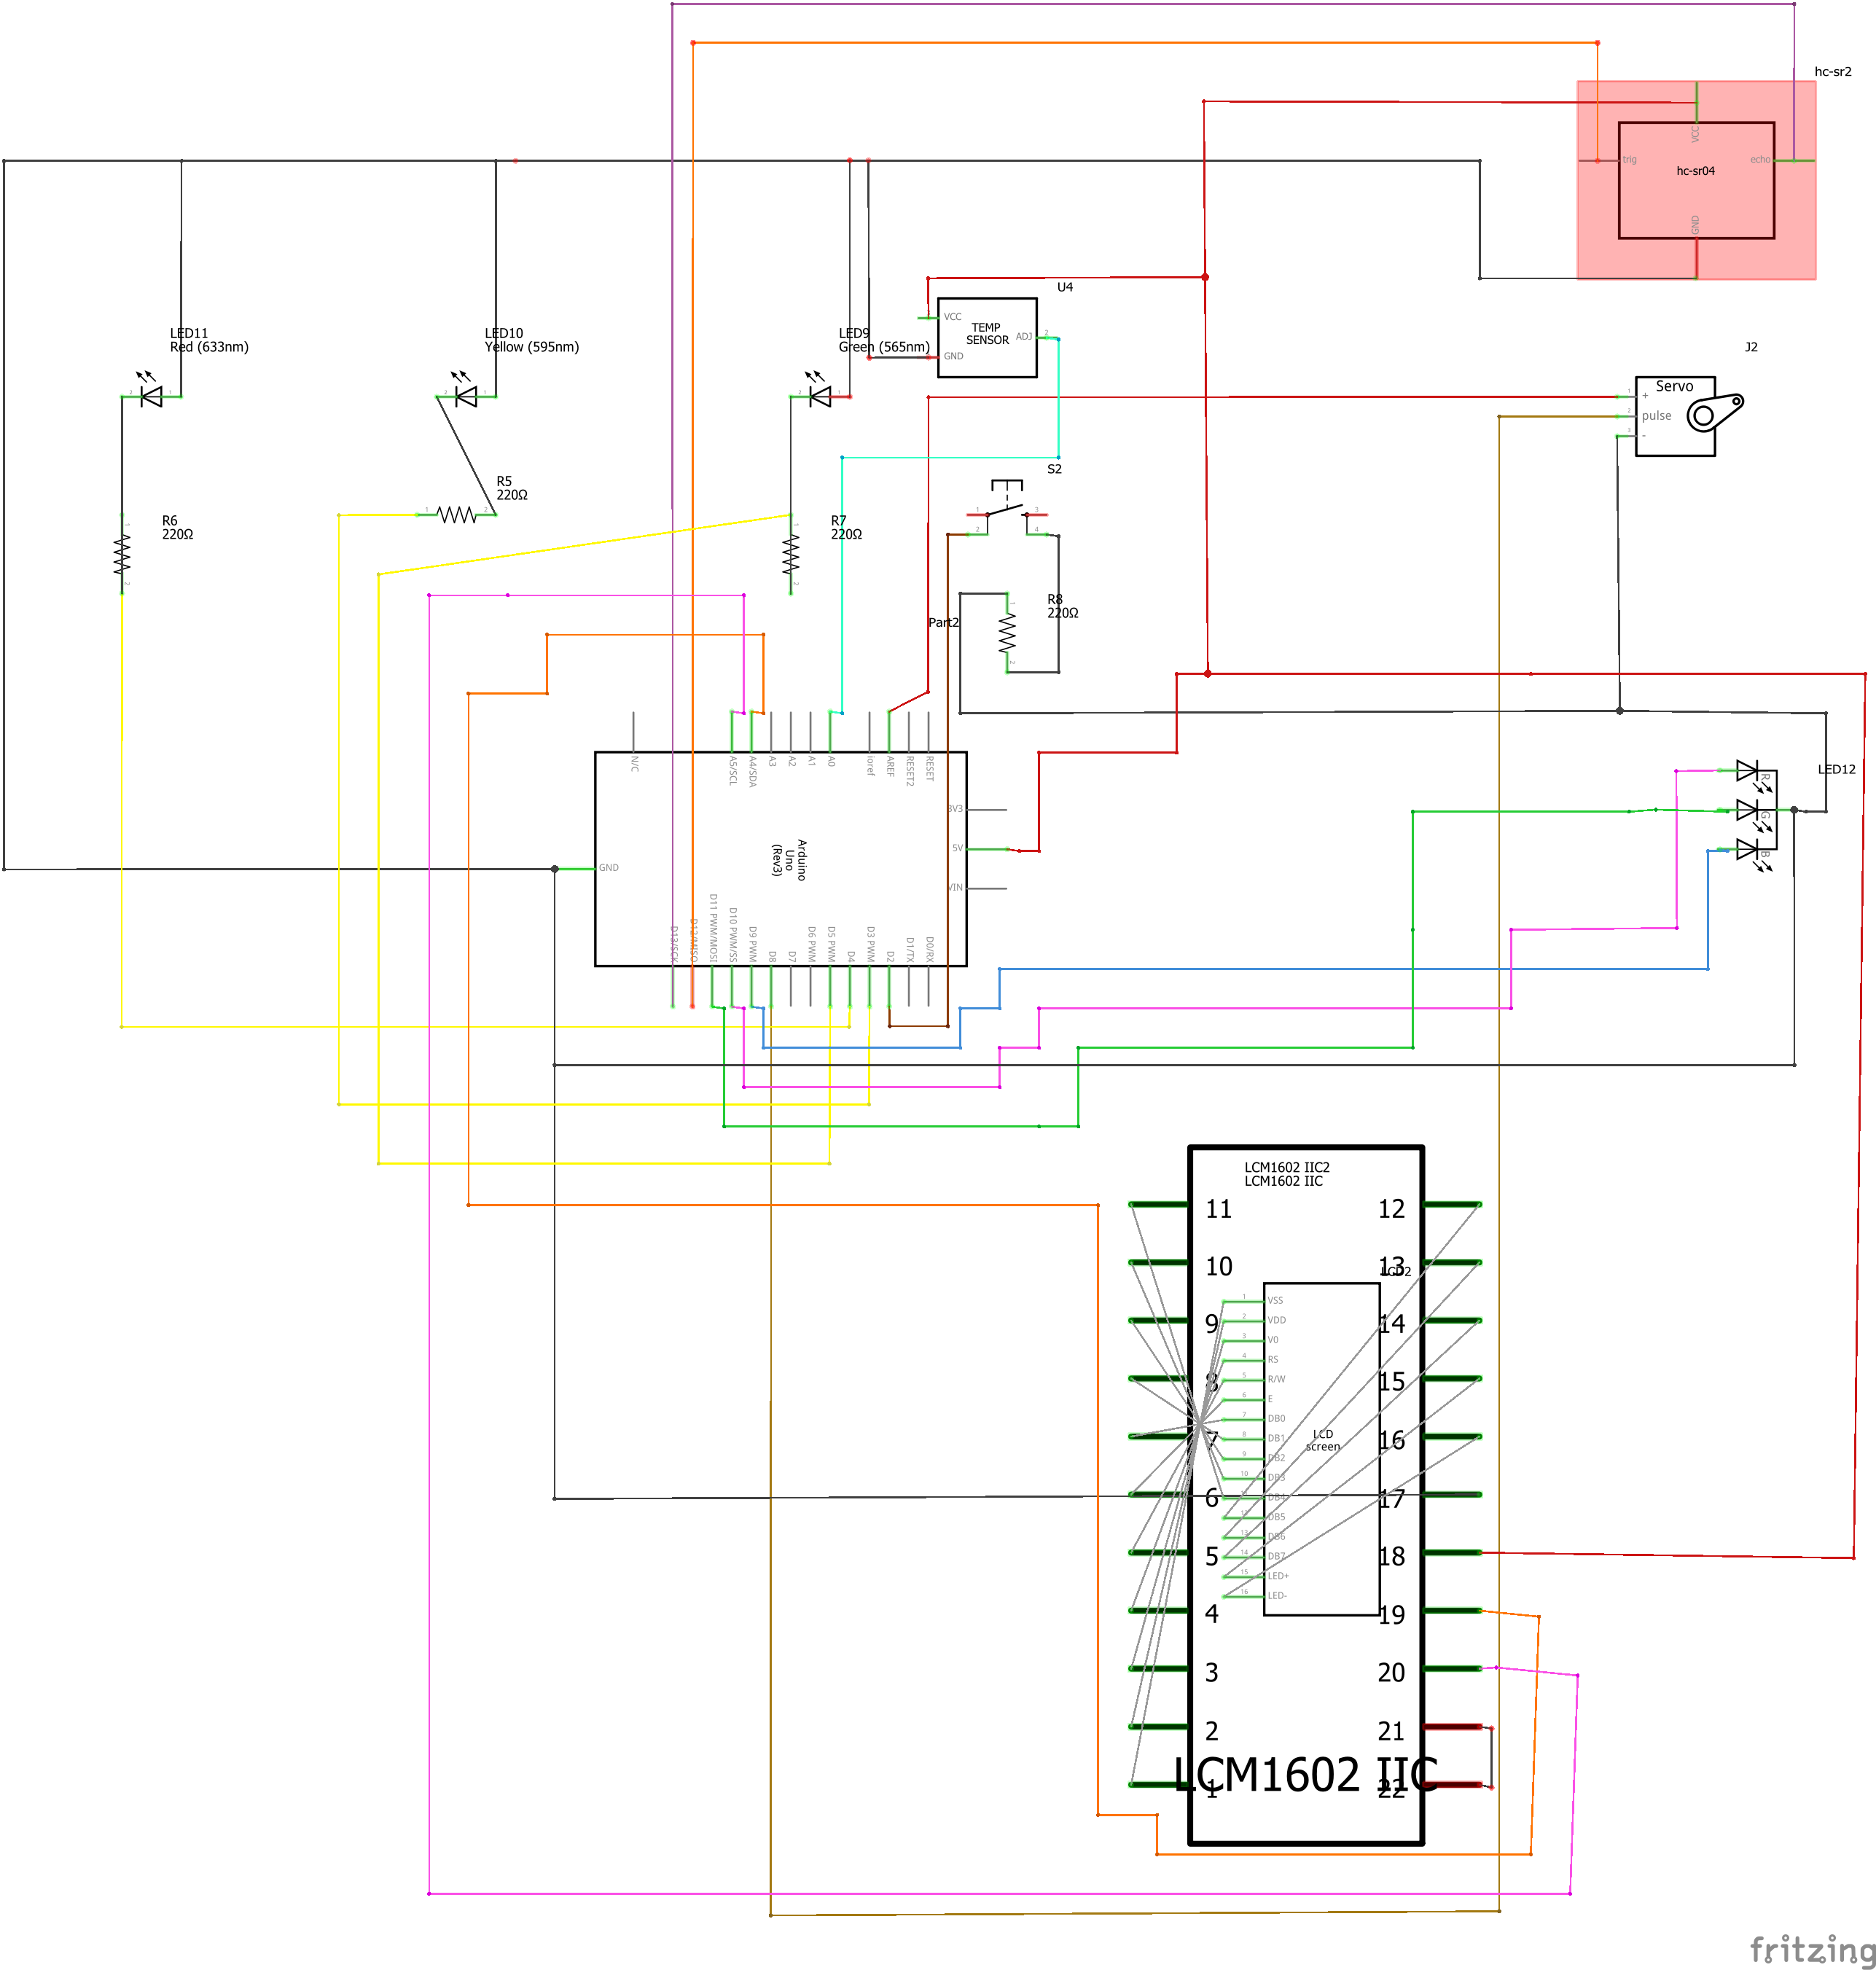
\includegraphics [width=\linewidth]{fig/Circuittekning}
  \caption{Circuit drawing}
  \label{fig:Circuitdrawing}
\end{figure}

As we can see the circuit board has been left out, and the individual components are all connected directly to the Arduino.  

OBS! The LCD display and the LCD controller are drawn as two components, but in this project they are one unit, so the non-important wires are grey, while the four wires connecting the LCD unit to the Arduino are the important ones. 